\chapter{\label{chap:CBIR}Recuperação de imagens pelo conteúdo}

A disseminação dos sistemas de hardware embarcado, com capacidade de coletar, armazenar e disponibilizar imagens digitais em redes de computadores, ampliou a demanda por aplicações de visão computacional em áreas como a medicina, industria, segurança e biologia para citar algumas. Dentre as demandas, há uma urgente por ferramentas efetivas de gerenciamento de informação multimídia que facilitem a organização e a busca automática desse tipo de conteúdo. 

Busca de imagens em grandes bases de dados multimídia é um dos serviços mais importantes disponibilizados pelos sistemas de gerenciamento de informação na atualidade. O método clássico para se prover tal serviço emprega a rotulação textual por palavras-chave. Nessa abordagem o usuário realiza buscas fornecendo informações textuais ao sistema. Esse último recupera a informação multimídia empregando métodos tradicionais de buscas textuais por palavras-chave. Atualmente essa abordagem tem se tornado inviável devido ao grande volume de informação multimídia disponível na internet, o que torna o processo de anotação textual demasiadamente dispendioso. Ademais o processo de descrição textual é impreciso, uma vez que diferentes indivíduos tendem a interpretar e descrever uma mesma imagem subjetivamente e, portanto, empregando diferentes palavras-chave na descrição.

Este capítulo trata dos sistemas de recuperação  de imagens pelo conteúdo (\emph{CBIR}). Nesses sistemas o processo de busca utiliza o conteúdo visual das imagens. A grande vantagem dos sistemas CBIR em relação aos sistemas que empregam rotulação textual é a não necessidade de anotação textual da informação.

\section{Arquitetura dos sistemas \emph{CBIR}}

Sistemas \emph{CBIR} empregam o conteúdo visual das imagens para formar uma base de dados de representações na forma de vetores de características. A busca é então realizada com o usuário fornecendo ao sistema uma imagem, ou figura de consulta, a qual também é representada vetorialmente. Assim, através da avaliação da similaridade existente entre as representações da imagem de consulta e das imagens da base, o sistema procura retornar ao usuário as imagens que sejam do seu interesse. Dependendo das particularidades da aplicação, esse padrão de consulta, que corresponde também a uma imagem, pode ser um esboço, um modelo ou uma cópia exata do que se deseja procurar \cite{Smeulders:2000}.

\begin{comment}
Sistemas \emph{CBIR} realizam buscas em bases multimídia utilizando o conteúdo visual das imagens, visando recuperar imagens que sejam do interesse do usuário mediante um padrão de consulta especificado. O campo das pesquisas em recuperação de imagens pelo conteúdo é vasto e relativamente recente.
\end{comment}


Na Figura \ref{fig:cbir} temos representada a arquitetura de um sistema \emph{CBIR} clássico, sendo este composto pelos seguintes componentes \cite{Torres:2006}:

\begin{alineas}
\item Módulo de interação com usuário: através desse módulo o usuário fornece como entrada ao sistema uma imagem de consulta e visualiza, como saída, os resultados das buscas. É também através desse módulo que são realizadas a inserção e a remoção de imagens da base de imagens, sendo esse último processo, destacado em linhas tracejadas, realizado pelo administrador do sistema;  
\item Módulo de processamento de busca: esse módulo engloba grande parte da funcionalidade do sistema \textit{CBIR}, sendo esse composto pelos seguintes sub-módulos:
\begin{alineas}
\item Extração de características: contempla os algoritmos computacionais responsáveis em obter uma representação matemática, na forma de vetor de características, dos atributos visuais das imagens como cor, textura e forma;
\item Avaliação de similaridade: contempla o método empregado para a avaliação do grau de similaridade existente entre as imagens a partir de suas respectivas representações vetoriais;
\item Ordenação dos resultados: método para seleção das imagens que serão apresentadas ao usuário conforme o grau de similaridade ao padrão fornecido;
\end{alineas} 
\item Base de imagens: repositórios aonde estão contidas as imagens, bem como suas correspondentes representações vetoriais.
\end{alineas}

\begin{figure} 
\centering
\caption{\label{fig:cbir} Arquitetura de um sistema \emph{CBIR}.}
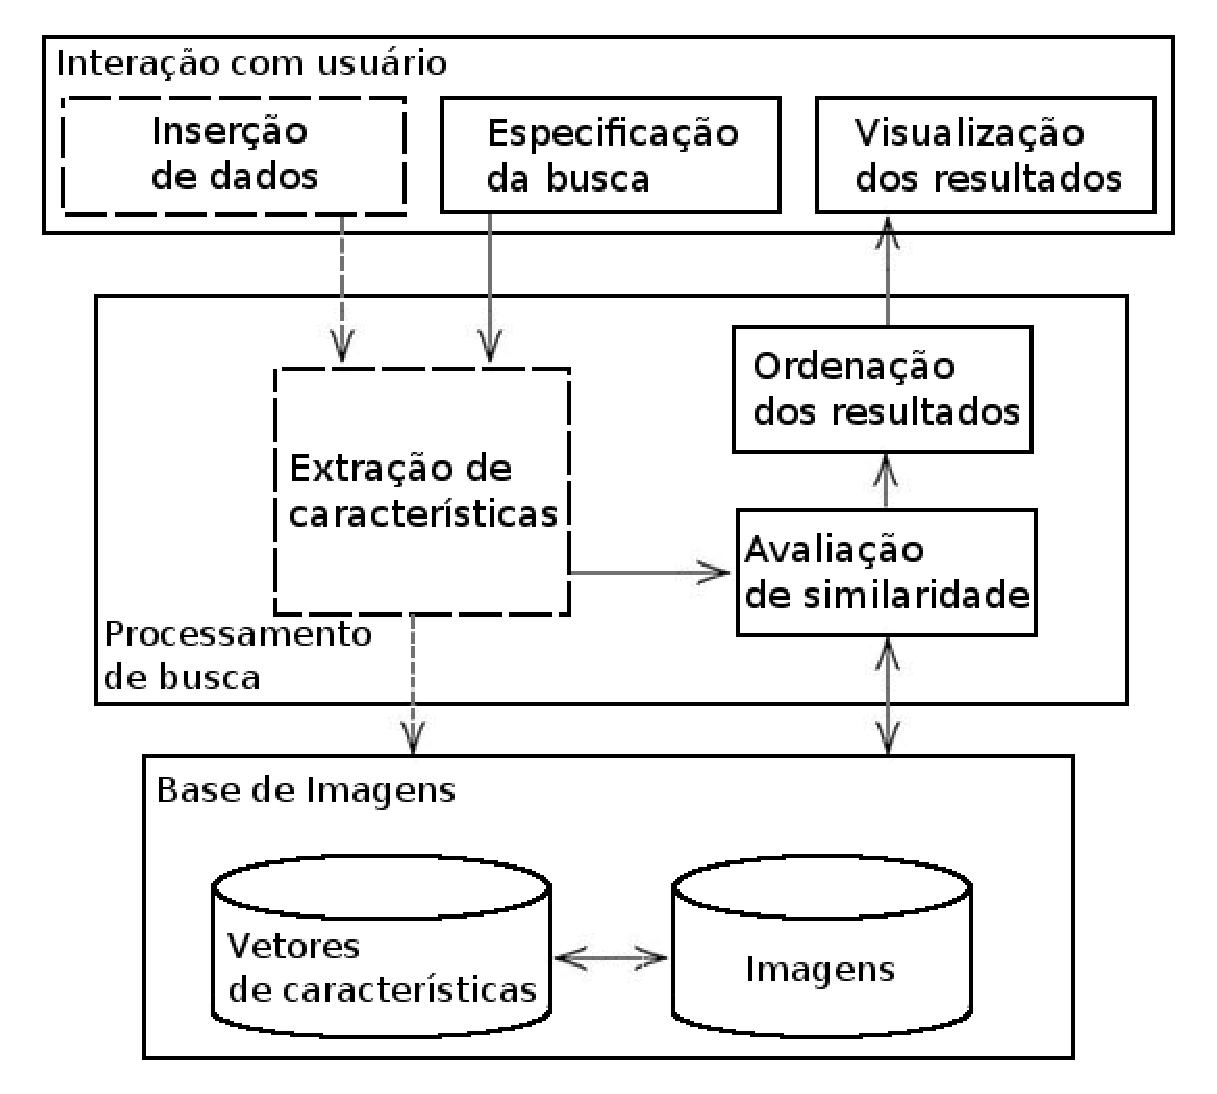
\includegraphics[width=0.65\textwidth]{cbir.eps}
\legend{Fonte: \citeonline{Torres:2006}.}
\end{figure}
 
Neste trabalho enfatizamos os processos de extração de características e de avaliação de similaridade em \emph{CBIR}, sendo esses processos destacados nas subseções a seguir.

\subsection{Extração de características}

Os estímulos visuais, ao qual os sistemas de visão biológicos estão submetidos, apresentam um elevado grau de redundância de informação. No processamento dessa informação, tais sistemas buscam eliminar essas redundâncias, retendo apenas a quantidade de informação necessária para o desempenho da tarefa requerida.  

Em visão computacional e reconhecimento de padrões, dá-se o nome a esse processo de eliminação das redundâncias de extração de características. Esta etapa de baixo nível busca encontrar informação relevante em uma imagem e representá-la convenientemente para a realização de uma tarefa específica de visão computacional. Uma vez que o processo de extração de características determina o desempenho de um sistema de visão computacional, este recebe especial atenção no desenvolvimento de tais sistemas.

Desta forma, o processo de extração de características das imagens, a fim de representá-las em um espaço vetorial $N$-dimensional, forma o alicerce dos sistemas \emph{CBIR}. Tal processo se dá através de operações de processamento de imagens, cujo objetivo é extrair informação que seja semanticamente relevante dos atributos da imagem para a realização das buscas. 

Os atributos comumente empregados para extração de características em \emph{CBIR} são a cor, a textura, a forma e a localização espacial dos elementos constituintes de uma imagem. 

A cor é o atributo mais empregado em \emph{CBIR}, pois a mesma permite discriminar uma ampla gama de imagens. Quando se utiliza esse atributo deve se considerar que o registro da cor em uma imagem varia consideravelmente com a orientação da superfície imageada, o posicionamento da câmera, a posição da fonte de iluminação e a maneira como a luz interage com os objetos imageados \cite{Smeulders:2000}. Ademais, a percepção humana da cor é um assunto complexo que ainda não está completamente elucidado \cite{Smeulders:2000}. De acordo com \citeonline{Torres:2006}, as técnicas de descrição por cores podem ser agrupadas em duas grandes classes dependendo se a informação de cor é codificada correlacionada com a sua distribuição espacial ou não. 

\begin{comment}Esses mesmos autores exemplificam como técnicas que não levam em consideração a distribuição espacial das cores os histogramas e os momentos de cores. 
\end{comment}

Atributos de textura são úteis na recuperação de imagens de satélites, bem como na busca de documentos digitalizados \cite{Smeulders:2000}. Essa é definida em termos de estruturas formadas por grupos de pixels que aparecem na imagem com certa periodicidade ou aleatoriedade. O método já consagrado para descrição de características de texturas é a matriz de co-ocorrência proposta por \citeonline{4309314}. No entanto, métodos baseados em transformações wavelet têm sido utilizados \cite{5376587}, mais notoriamente a transformada wavelet de Gabor \cite{531803}. Outra técnica que tem sido explorada na atualidade para descrição de texturas é a dimensão fractal multiescala \cite{Florindo:2013-2}. 

\subsection{Medidas de similaridade}
O processo de recuperação de imagens pelo conteúdo requer que alguma medida seja empregada na avaliação da similaridade entre as representações das imagens. Uma vez que as técnicas de extração de características resultam em representações vetoriais, as medidas de dissimilaridade entre vetores são comumente empregadas para este fim. Desta forma, o grau de similaridade entre duas representações guarda uma relação inversa com a medida de dissimilaridade correspondente. 

Uma medida de dissimilaridade é considerada uma métrica de distância quando satisfaz as seguintes propriedades: 

\begin{alineas}
\item Positividade: $d(p,q) \geq 0$;  
\item Unicidade: $d(p,q) = 0 \Rightarrow p = q$;
\item Simetria: $d(p,q) = d(q,p)$;
\item Desigualdade triangular: $d(p,r) + d(r,q) \geq d(p,q)$.
\end{alineas}

Para as representações vetoriais dentro de um mesmo espaço dimensional, distâncias simples entre vetores, de baixo custo computacional, como as apresentadas na Tabela \ref{tbl:distance}, são empregadas. Já nos casos aonde a representação das imagens resulta em representações de dimensões distintas, técnicas mais elaboradas, e portanto de maior custo computacional, são empregadas para avaliação de distância. Dentre essas técnicas a \emph{DSW} (\emph{Dynamic space warping}), empregada na comparação de séries temporais, tem sido empregada na avaliação de similaridade entre formas a partir de assinaturas extraídas dos seus contornos \cite{Alajlan20117}. 

\begin{table}
\centering
\caption{\label{tbl:distance}Medidas de dissimilaridade entre vetores}
\begin{tabular}[]{ll}
\hline
Medida de dissimilaridade&Fórmula matemática\\
\hline
Distância de Minkowski&$d(x,y) = \Big[\sum\limits_{i=1}^{n}(x_i-y_i)^m\Big]^\frac{1}{m}$\\
Distância euclidiana&$d(x,y) = \Big[\sum\limits_{i=1}^{n}(x_i-y_i)^2\Big]^\frac{1}{2}$\\
Distância city-block&$d(x,y)= \sum\limits_{i=1}^{n}|x_i-y_i|$\\
Distância Chebyshev&$d(x,y)= \max\limits_{i}|x_i-y_i|$\\
Separação angular&$d(x,y)=\frac{\sum\limits_{i=1}^n{x_iy_i}}{\Big[\sum\limits_{i=1}^n{x_i^2}\sum\limits_{i=1}^n{y_i^2}\Big]^\frac{1}{2}}$\\
Canberra&$d(x,y) = \sum\limits_{i=1}^n\frac{|x_i-y_i|}{x_i+y_i}$\\
\hline
\end{tabular}
\end{table}

\begin{comment}
\section{\emph{Gap semântico}}
Uma questão importante nos sistemas \emph{CBIR} é que, embora os usuários busquem por imagens similares do ponto de vista semântico, o sistema provê os resultados com base na similaridade da informação extraída do conteúdo visual das imagens. A disparidade existente entre esses aspectos (semântica e conteúdo visual) é denominado de \emph{Gap} semântico.

Embora as imagens transmitam determinadas mensagens ao usuário, muito frequentemente os atributos extraídos das mesmas não conseguem representar e caracterizar essas mensagens. Diversos métodos para associar informação semântica aos atributos extraídos das imagens têm sido foco de pesquisa, como por exemplo solicitar que o usuário retro-alimente o sistema com o grau de relevância dos resultados obtidos (relevance feedback). 

\section{Base de imagens}

Um aspecto importante em \emph{CBIR} está ligado ao mecanismo de indexação empregado no acesso a informação contida na base de imagens. Em aplicações práticas, que requerem acesso a uma extensa base de dados, e aonde há interação dos usuários com o mecanismo de busca, o desempenho computacional no processo de indexação não pode ser negligenciado. Desta forma, armazenar vetores de características em um arquivo linear, com um registro para cada vetor, resulta na indexação sequencial destes elementos tornando essa abordagem inviável.

Todavia, mecanismos alternativos de indexação tradicionalmente encontrados na literatura, tais como \emph{k-d-b tree}, \emph{quad-tree} e \emph{R-tree} são considerados inadequados em \emph{CBIR} porque o desempenho destes se degrada substancialmente com o amumento da dimensionalidade dos dados. Ademais, para alcançar a eficiência computacional requerida sem degradar a qualidade das buscas, tais mecanismos devem levar em consideração a representação das características das imagens no processo de recuperação, ou seja, não só apenas \emph{como} indexar elementos na base de dados, mas também \emph{o que} indexar.

\end{comment}

\chapter{\label{chap:contour}Características do contorno das formas}

Dentre os atributos dos quais se realizam a extração de características, a forma é considerada a mais relevante em diversas aplicações de visão artificial pela riqueza de informações que esta possui. Uma forma é obtida quando um objeto de interesse é identificado e segmentado em uma imagem. 
 De acordo com \citeonline{Zhang:2004}, para que se obtenha uma representação conveniente com base nesse atributo, deve-se buscar por informações que tenham importância em sua percepção, seja no contorno ou na região que a delimita. 

Obter uma representação, ou descrição, a partir de formas planas é uma tarefa complexa. Isso porque quando projetamos objetos tridimensionais do mundo real em duas dimensões, perdemos as informações de uma das dimensões. Como resultado temos uma representação bidimensional parcial do objeto projetado. O problema torna-se ainda mais complexo se levarmos em conta que a forma é frequentemente corrompida por ruídos, defeitos, distorções arbitrárias e oclusões.

\citeonline{Zhang:2004} classificam as técnicas de representação de formas em duas grandes classes de métodos: os baseados em contorno e os baseados em região. Nos métodos baseados em região as características são extraídas de toda região da forma. Já nos métodos baseados em contorno as características são extraídas apenas da borda. Os referidos autores ainda subdividem cada classe de métodos em métodos estruturais e globais. Essa subdivisão é baseada em se a forma como um todo é utilizada na representação ou se a representação é obtida de partes, segmentos e seções das formas. Este trabalho de pesquisa enfatiza a aplicação de técnicas de processamento de sinais para a obtenção de representações globais do contorno das formas. 

\begin{comment}
Técnicas baseadas em contorno de formas exploram apenas a região da borda da forma. Há dois tipos de abordagens para extração de características do contorno das formas: global e estrutural. Na abordagem global a forma não é dividida em sub-partes e um vetor de características que representa toda a borda é obtido para representar a forma. Na abordagem estrutural a borda da forma é particionada em segmentos, denominados de primitivas mediante algum critério. A representação final é geralmente uma cadeia de caracteres, um grafo ou uma árvore.
\end{comment}

Técnicas de processamento de sinais têm sido empregadas com sucesso na obtenção de representações a partir do contorno das formas \cite{Costa:2009}. A Figura \ref{fig:folha_contorno1} ilustra as etapas envolvidas nesse processo. Temos nesse caso a segmentação da imagem por limiar seguida da extração do contorno. Com base no contorno, consegue-se obter uma variedade de representações, na forma de sinais, adequadas para as tarefas de comparação, classificação e reconhecimento de formas. Neste capítulo apresentamos algumas dessas representações. 

%representar uma forma consiste em caracterizá-la através de um conjunto de características que permitam reconstruir-la exatamente ou com um certo grau de precisão. Os mesmos autores classificam os métodos de representação das formas em três grandes grupos: por contorno, por região e por transformação.
    

\begin{figure} 
\caption{\label{fig:folha_contorno1} Obtenção da forma e do contorno da imagem de uma folha.}
%\includegraphics[width=\textwidth,clip,trim=12mm 188mm 27mm 75mm]{figura_folha.png}
\includegraphics[width=\textwidth,clip,trim=10mm 145mm 36mm 26mm]{figura_folha.png}
\end{figure}

\section{Representações paramétricas}\label{sec:Rep_par}
A representação paramétrica consiste nas coordenadas dos pontos amostrados do contorno, representados a partir de um sistema de coordenadas pré-estabelecido, percorrendo-o sequencialmente em sentido horário ou anti-horário. Para o contorno discreto $\mathbf{C}$, com $N$ amostras, representado num sistema de coordenadas cartesianas, tal processo origina um conjunto de tuplas $\mathbf{C}[n] = \big(\mathbf{X}[n]\:\text{,}\:\mathbf{Y}[n]\big)$, $n \in {\{0\:\text{,}\:1\:\text{,}\:\dotsc\:\text{,}\:N-1\}}$, cujas componentes $\mathbf{X}[n]$ e $\mathbf{Y}[n]$ são sinais discretos vetoriais das coordenadas amostradas do contorno.

Na Figura \ref{fig:folha_contorno} estão representados os sinais obtidos para o contorno da folha da Figura \ref{fig:folha_contorno1} com a amostragem $N = 280$ pontos. Em vermelho está destacado o ponto de origem aonde a varredura, em sentido horário, se inicia. Os dois pontos observados aonde a evolução do sinal $\mathbf{Y}[n]$ inverte sua tendência (de crescente para decrescente e de decrescente para crescente) correspondem aos pontos mais salientes da folha. Já o platô observado no sinal $\mathbf{X}[n]$ corresponde a região da parte inferior da folha, em que quase não se observa variações do contorno ao longo do eixo $X$.
   
\begin{figure} 
\caption{\label{fig:folha_contorno} Processo de obtenção da representação paramétrica do contorno da folha da Figura \ref{fig:folha_contorno1}.}
\includegraphics[width=\textwidth,clip,trim= 12mm 23mm 10mm 77mm]{figura_folha.png}
\end{figure}

Outra representação paramétrica para o contorno é obtida compondo-se um sinal complexo $\mathbf{z}[n] = \mathbf{X}[n] + j\mathbf{Y}[n]$, $j = \sqrt{-1}$, $n \in {\{0\:\text{,}\:1\:\text{,}\:\dotsc\:\text{,}\:N-1\}}$. Essa representação é conveniente quando se deseja realizar extração de características do contorno através de operações de processamento de sinais. A Figura \ref{fig:folha_complex} ilustra o módulo e a fase da representação complexa do contorno da folha da Figura \ref{fig:folha_contorno1}. 

\begin{figure} 
\caption{\label{fig:folha_complex} Representação paramétrica do contorno da folha da Figura \ref{fig:folha_contorno1} como sinal complexo.}
\includegraphics[width=\textwidth]{folha_complex_v2.png}
\end{figure} 

As representações paramétricas são consideradas representações intermediárias, uma vez que não apresentam propriedades de invariância à translação, escalamento e espelhamento das formas \cite{Kindratenko:2003}. No entanto, importantes propriedades geométricas da forma, que permitem construir descritores com as propriedades de invariância mencionadas, podem ser obtidas com base nestas representações, como o perímetro do contorno, área da forma, curvatura, dentre outras \cite{Kindratenko:2003}.

\section{\label{sec:Assinatura}Representação por assinaturas}

Embora sejam descritivas, as representações apresentadas na Seção \ref{sec:Rep_par} apresentam o inconveniente de não serem invariantes a translação, rotação ou escalamento das formas. Partindo-se de tais representações, podem ser obtidas assinaturas que apresentem algumas das propriedades de invariância supracitadas.

\citeonline{Costa:2009} definem assinatura de uma forma como sendo um sinal discreto uni-dimensional que descreve algumas das características do seu contorno ou da sua região. Devido a redução de dimensionalidade, as assinaturas do contorno são representações compactas das formas. 

Estas podem ser utilizadas diretamente como descritores, porém o custo computacional envolvido em sua comparação direta é elevado. Isso porque as assinaturas frequentemente não são totalmente insensíveis a rotação, translação e escalamento das formas, bem como variam no total de amostras conforme varia a resolução das imagens. 

Algumas assinaturas são mais sensíveis a ruído e a pequenas distorções dos contornos, tornando necessário realizar filtragens. Embora melhore a robustez, tal processo acarreta em alguma perda de informação.

Várias assinaturas vêm sendo empregadas na literatura para descrição de formas nas mais diversas aplicações, tais como a distância ao centróide, as coordenadas complexas, ângulo tangente, ângulo acumulativo, curvatura, área e comprimento da corda \cite{Zhang:2004}.


\subsection{Curvatura}\label{sec:curvatura}

A curvatura é uma assinatura obtida a partir do contorno com importantes propriedades geométricas, o que motiva sua utilização para obtenção de descritores de formas. Há evidências biológicas de que as propriedades desta assinatura sejam exploradas pelo sistema de visão dos primatas nas tarefas de reconhecimento de formas. Na Tabela \ref{tbl:curv} estão destacadas as principais propriedades que a curvatura apresenta.  

\begin{table}
\centering
\caption{\label{tbl:curv} Propriedades da curvatura e as características geométricas que essas representam.}
\begin{tabular}[]{ll}
\toprule
\multicolumn{1}{c|}{Propriedade} & \multicolumn{1}{c}{Característica da forma}\\ 
\hline
Máximo valor absoluto & Ponto saliente \\
Máximo valor positivo & Saliência convexa \\
Mínimo valor negativo & Saliência côncava \\
Valores constantes e nulos & Segmentos retilíneos \\
Valores constantes e não nulos & Segmentos circulares \\
Cruzamentos de zero & Pontos de inflexão \\ \bottomrule
\end{tabular}
\end{table}

Sua função $k(l)$, para uma curva contínua fechada $C = \big(x(l)\:\text{,}\:y(l)\big)$,  cujo perímetro é $L$ e que encontra-se parametrizada em $l \in [0\text{,}L]$, é definida como sendo \cite{Kindratenko:2003}:

\begin{equation} \label{eq:curvatura}
k(l) = \frac{x^{'}(l)y^{''}(l)-x^{''}(l)y^{'}(l)}{((x^{''}(l))^{2}+(y^{''}(l))^{2})^{\frac{3}{2}}}
\end{equation}

, sendo $\big(x^{'}(l) \text{, }y^{'}(l)\big)$ e $\big(x^{''}(l)\text{ , }y^{''}(l)\big)$ as derivadas primeira e segunda das coordenadas paramétricas da curva, respectivamente.

Sob o aspecto computacional, o cálculo da curvatura do contorno de uma forma,  requer que o mesmo seja espacialmente amostrado e discretizado. Tal processo torna o cálculo das derivadas da Equação \ref{eq:curvatura} extremamente ruidoso e inviável, o que limita a aplicação direta da curvatura para a obtenção de descritores. 

Na Figura \ref{fig:cir1} temos a ilustração de tal efeito para uma imagem de forma circular. A esquerda está representado o gráfico da curvatura teórica, obtida analiticamente, pela aplicação da equação \ref{eq:curvatura} ao contorno parametrizado de um círculo de mesmo raio que o círculo da imagem central. Já a direita, temos a curvatura obtida computacionalmente a partir do contorno discreto do círculo da imagem no centro da referida figura. Nota-se no gráfico que a curvatura teórica (à esquerda) tem um valor constante $k(l) = \frac{1}{r}$, sendo $r$ o raio do círculo, enquanto que na curvatura obtida computacionalmente ocorrem variações significativas em torno do valor teórico esperado.

\begin{figure}[h!]
  \caption{\label{fig:cir1} Efeito do ruído na estimativa computacional da curvatura para uma forma circular.}
  \centering
  \includegraphics[width=\textwidth]{curv_cir.png}
\end{figure}

Diversas estratégias foram propostas na literatura para contornar o problema da sensibilidade a ruído do cálculo computacional da curvatura. Trabalhos clássicos, como os de \citeonline{5009188} e \citeonline{LynnBeus1987291} buscam estimar a curvatura a partir do ângulo formado entre vetores obtidos a partir dos pontos do contorno. Já \citeonline{Cazals:2003} e \citeonline{Shi20022051} apresentam trabalhos que utilizam métodos para estimação da curvatura por interpolação de pontos. 

\citeonline{149591} apresentam um método que suaviza o contorno, através da convolução do mesmo com um filtro passa-baixas gaussiano, antes de se calcular a curvatura.

\begin{figure}[h!]
 \caption{\label{fig:curv_folha} Curvatura estimada do contorno da folha da Figura \ref{fig:folha_contorno1} através de método computacional.}
  \centering
  \includegraphics[width=\textwidth]{curv_folha_v2.png}
\end{figure}

A Figura \ref{fig:curv_folha} mostra a curvatura estimada, para o contorno da folha da Figura \ref{fig:folha_contorno1}, através desse último método. O contorno foi previamente suavizado com um filtro gaussiano com desvio padrão $\sigma = 20$. Os pontos aonde a curvatura apresenta os picos em destaque correspondem aos pontos salientes da folha. 

\begin{comment}
Particularmente, métodos de extração de características multiescala do contorno a partir da curvatura conseguem superar o problema supracitado aplicando filtragens passa-baixa a representação paramétrica do contorno antes de se calcular a curvatura. 
\end{comment}

\subsection{Distância ao centróide}
Uma assinatura simples pode ser obtida calculando-se a distância de cada coordenada do contorno ao centróide da forma. Esse último consiste, para um contorno discreto de $N$ amostras, em um vetor calculado, a partir das coordenadas do contorno, pela seguinte equação: 

\begin{equation}
\big(X_{c}\:\text{,}\:Y_{c}\big) = \Big(\frac{1}{N}\sum^{N}_{i=0}{X[i]}\:\text{,}\:\frac{1}{N}\sum^{N}_{i=0}{Y[i]}\Big)
\end{equation}

A distância ao centróide $dc[n]$ é dada por:

\begin{equation}
dc[n] = \sqrt{(X[n] - X_c)^2 + (Y[n] - Y_c)^2}
\end{equation}

Essa assinatura tem a propriedade de ser invariante a translação da forma, o que a torna independente do sistema de coordenadas adotado na parametrização do contorno. Embora não seja invariante a escala e a rotação, tais invariâncias podem ser obtidas, como sugerem alguns trabalhos. 

Empregando um processo de sub-amostragem e de normalização pelo maior valor, \citeonline{Wang:2000} tornam essa assinatura invariante a escala. Para se alcançar invariância a rotação os referidos autores sugerem que, no processo de avaliação de similaridade entre duas assinaturas, seja realizado o deslocamento cíclico de uma das assinaturas até que se obtenha a maior similaridade.

Já \citeonline{Zhang:02} utilizam a distância ao centróide como assinatura para se obter os descritores de Fourier. Tal estratégia garante as propriedades de invariância a rotação e a escala.

\begin{figure}[h!]
  \caption{\label{fig:cd} Assinatura da distância ao centróide para o contorno da folha da Figura \ref{fig:folha_contorno1}}
  \centering
  \includegraphics[width=\textwidth]{cd_v2.png}
\end{figure}

A Figura \ref{fig:cd} ilustra a assinatura da distância ao centróide para a folha da Figura \ref{fig:folha_contorno1}. Neste exemplo, a assinatura foi normalizada a partir da distância máxima ao centróide, que corresponde ao ponto vermelho demarcado tanto no gráfico como no contorno. 

\subsection{Sequência de ângulos}

A sequência de ângulos é uma assinatura obtida a partir do ângulo formado entre vetores construídos a partir das coordenadas do contorno parametrizado conforme ilustrado na Figura \ref{fig:angulo}. 

Para um dado ponto pertencente ao contorno, de coordenadas $(x_i\:\text{,}\:y_i)$, obtemos os vetores $\overrightarrow{v_1}$ e $\overrightarrow{v_2}$. O primeiro vetor é formado pela diferença entre as coordenadas $(x_i\:\text{,}\:y_i)$ e $(x_{i-p}\:\text{,}\:y_{i-p})$, enquanto o segundo vetor é formado pela diferença entre as coordenadas $(x_{i+p}\:\text{,}\:y_{i+p})$ e $(x_i\:\text{,}\:y_i)$. 

Da propriedade do produto interno, temos a seguinte relação dessas coordenadas com o ângulo $\theta_i$, formado entre os vetores $\overrightarrow{v_1}$ e $\overrightarrow{v_2}$:

\begin{equation}
\overrightarrow{v_1}. \overrightarrow{v_2} = |\overrightarrow{v_1}||\overrightarrow{v_2}|\cos{\theta_i}=(x_i-x_{i-p})(x_{i+p}-x_i)+(y_i-y_{i-p})(y_{i+p}-y_i).
\end{equation}

Logo, o ângulo $\theta_i$ é calculado através da seguinte expressão:

\begin{equation}
\theta_i = \arccos{\Big[\frac{(x_i-x_{i-p})(x_{i+p}-x_i)+(y_i-y_{i-p})(y_{i+p}-y_i)}{\sqrt{\big[(x_i-x_{i-p})^2+(y_i-y_{i-p})^2\big]\big[(x_{i+p}-x_i)^2+(y_{i+p}-y_i)^2\big]}}\Big]}
\end{equation}

O parâmetro $p$ controla a sensibilidade da assinatura a características locais do contorno. Valores grandes desse parâmetro resultam em uma assinatura menos sensível a características locais, enquanto que valores pequenos fazem com que a assinatura seja mais sensível a características locais. 

A assinatura sequência de ângulos é empregada  para identificação de espécies vegetais a partir do contorno das folhas.

\begin{figure}[h!]
  \caption{\label{fig:angulo} Ilustração geométrica do método de obtenção da assinatura de sequência de ângulos.}
  \centering
  \includegraphics[width=0.35\textwidth]{angulo.png}
\end{figure}

\subsection{Invariantes integrais}

Uma vez que as assinaturas obtidas através de operadores diferenciais são sensíveis a ruídos e a pequenas deformações do contorno, \citeonline{Manay:2006} propuseram os invariantes integrais como uma representação inerentemente robusta a estes artefatos.

Seja $C \subset \mathbb{R}^2$ um contorno fechado e $\overline{C}$ sua área interior.
A função 

\begin{equation}
 B_r(p,x) = \left\{
  \begin{array}{l l}
    1 & \quad |p-x|\leq r\\
    0 & \quad |p-x|> r
  \end{array} \right.
\end{equation} indica se um ponto $x$ pertence ou não ao interior de um disco $B_r$,  centrado em $p$ e de raio $r$.

Empregando a função acima especificada, obtém-se uma assinatura invariante integral através da seguinte equação: 

\begin{equation}
A(p) = \int_{\overline{C}}{B_r(p,x)dx}
\end{equation}, sendo $p \in [0,L]$ e $L$ o perímetro do contorno.

A Figura \ref{fig:Aii} ilustra, do ponto de vista geométrico, o processo de obtenção da assinatura invariante integral. O disco $B_r(p)$ é centrado em cada ponto $p(s)$ pertencente ao contorno e a área de interseção entre $B_r(p)$ e a região interna ao contorno $\overline{C}(s)$ é determinada.

\begin{figure}[h!]
  \caption{\label{fig:Aii} Ilustração geométrica do método de obtenção da assinatura invariante integral.}
  \centering
  \includegraphics[width=0.75\textwidth]{aii.png}
  \legend{Fonte: \citeonline{Manay:2006}}
\end{figure}

\section{Representações multiescala} \label{chap:multiescala}

Qualquer método que se proponha a descrever características das formas com base em contornos deve ser capaz de representá-las de forma confiável e precisa. 

\begin{comment}Segundo \citeonline{149591}, esses devem satisfazer os seguintes requisitos:

\begin{alineas}
\item Invariância: duas curvas que tenham a mesma forma devem ter a mesma representação;
\item Unicidade: duas curvas que não tenham a mesma forma devem apresentar diferentes representações;
\item Estabilidade: pequenas variações observadas entre duas curvas devem resultar em pequenas variações em suas representações;
\item Eficiência: uma vez que alguns sistemas de visão computacional apresentam requisitos de tempo real, a descrição deve ser computacionalmente eficaz, demandando poucos recursos de memória e de processamento;
\item Fácil implementação: é recomendável que os métodos de descrição sejam simples e de fácil implementação de modo a requerer menos tempo de implementação e depuração; 
\item Relação com propriedades específicas das formas: o método de descrição deve ser capaz de representar propriedades das formas que este descreve.
\end{alineas}

Os referidos autores afirmam que muitos dos métodos de extração encontrados em visão computacional falharam em satisfazer um ou mais dentre estes requisitos.
\end{comment}

Embora carregue grande parte da informação a respeito das formas, o contorno é  sensível a ruídos, oclusões e variações das formas.  Em outros casos, o contorno não se apresenta completamente disponível, com regiões disjuntas e descontinuidades. Tais aspectos comprometem a confiabilidade e a precisão das assinaturas baseadas em contorno.  

A descrição multiescala do contorno das formas vêm se mostrando uma alternativa viável para superação de tais problemas. 

Esta técnica se baseia no método proposto por \citeonline{Witkin:1983} e \citeonline{Koenderink:1984} para análise de sinais em vários níveis de resolução. Esses autores introduziram o conceito de fator de escala, cujo ajuste determina o grau de resolução na qual ocorre a análise do sinal. 

\begin{figure}[h!]
  \caption{\label{fig:ms} Método de análise multiescala a partir da assinatura do contorno de uma forma.}
  \centering
  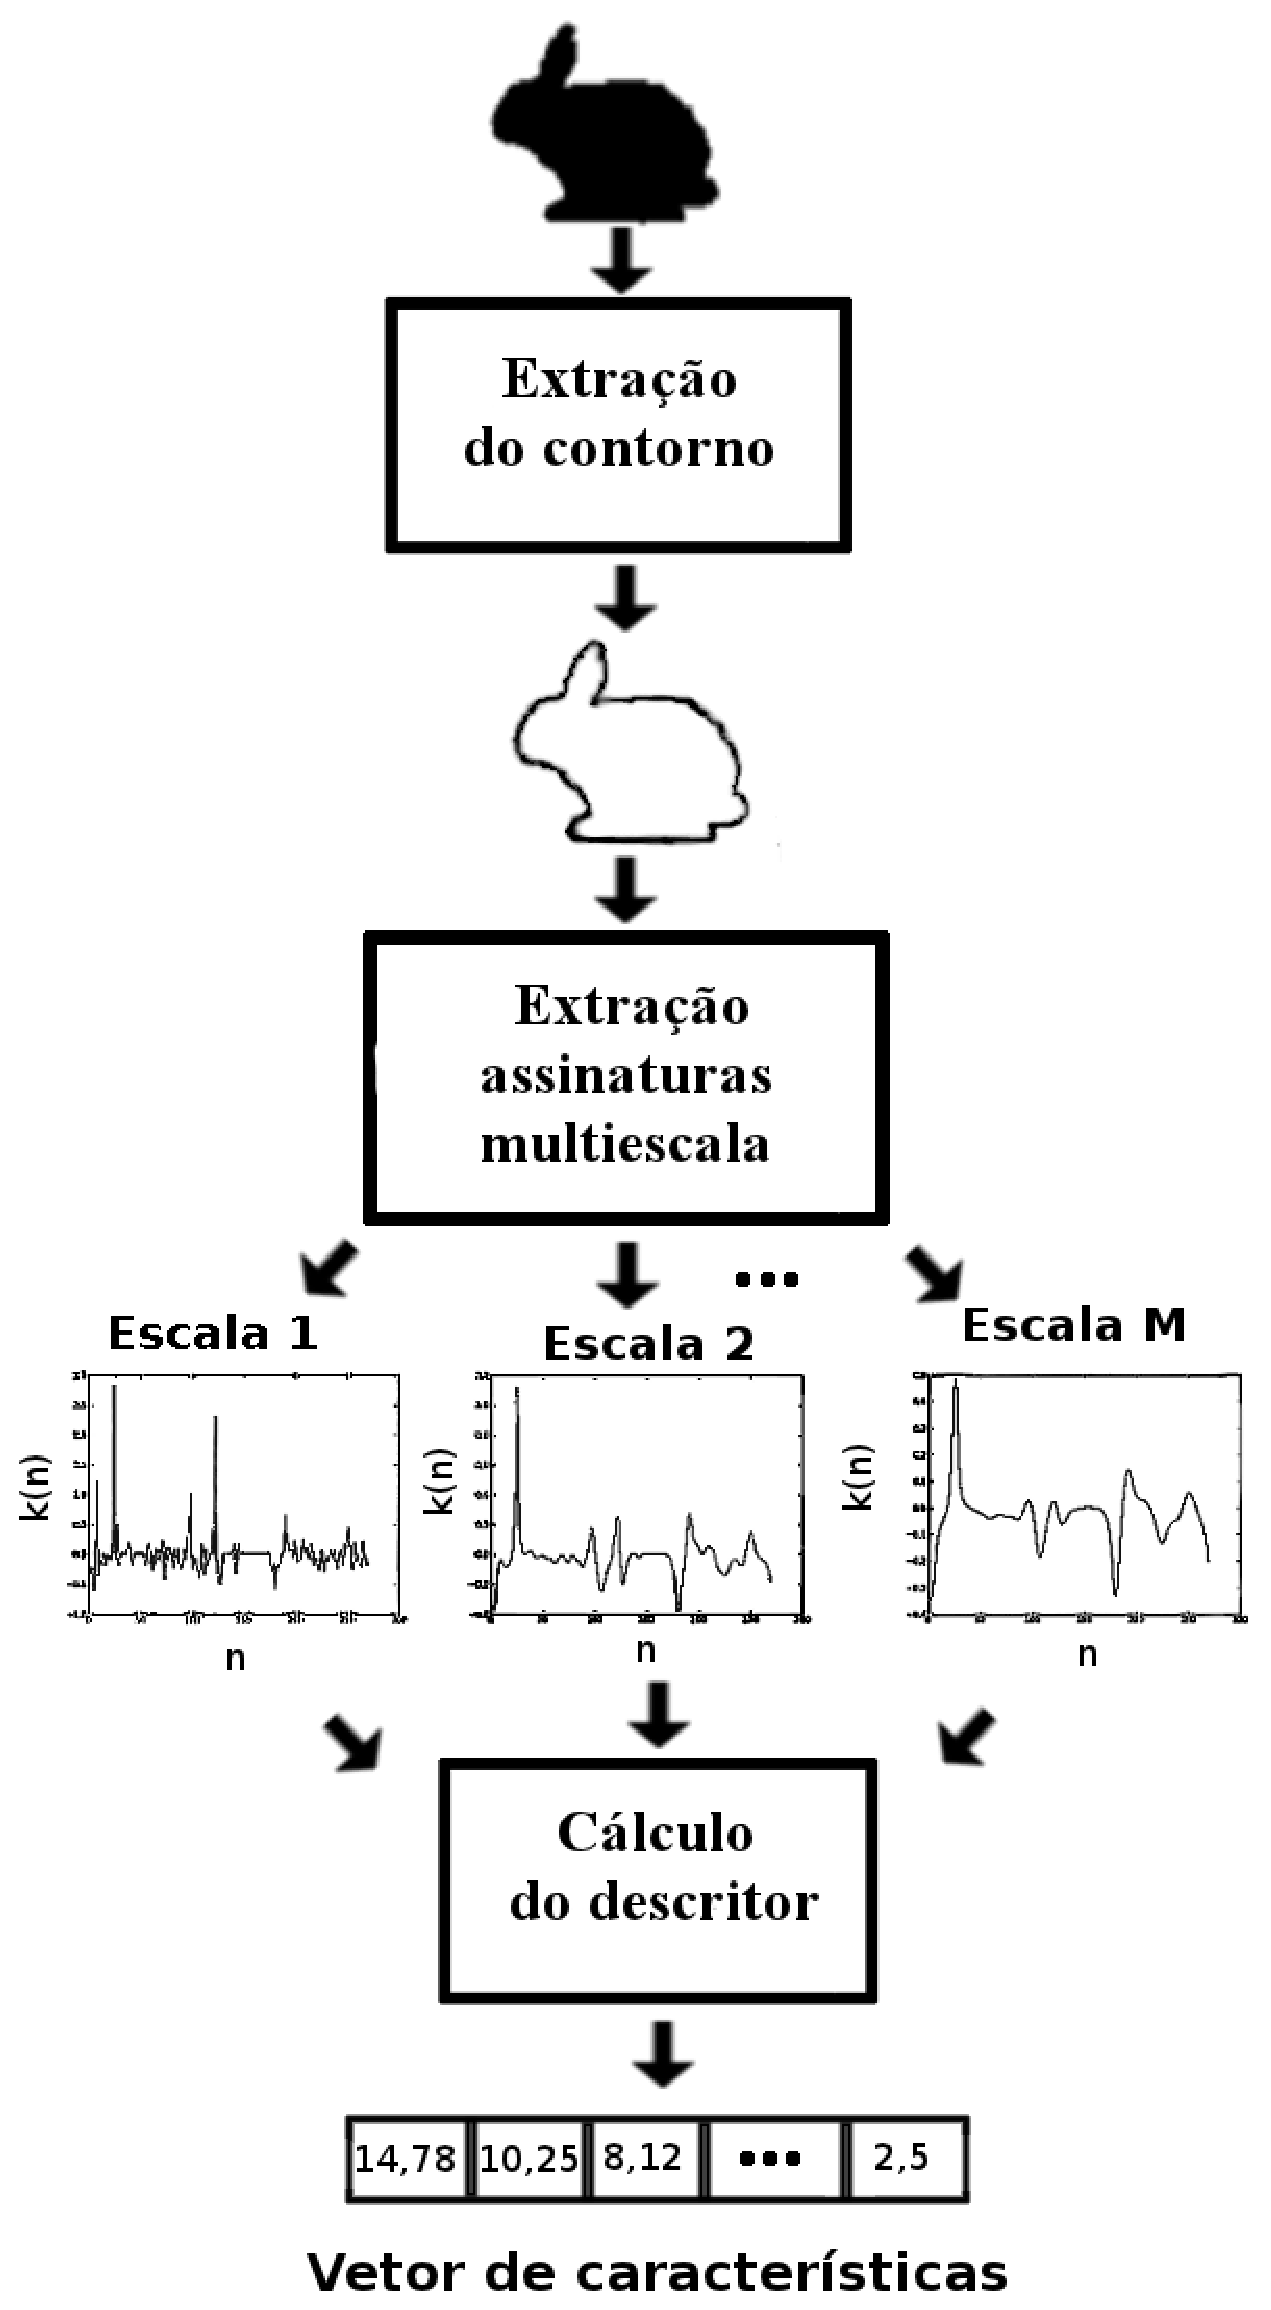
\includegraphics[width=0.45\textwidth]{feature_extraction.eps}
\end{figure}

A Figura \ref{fig:ms} ilustra o processo para obtenção de uma representação multiescala de um sinal unidimensional $u(t)$ que represente o contorno de uma forma, tal como as assinaturas apresentadas na Sessão \ref{sec:Assinatura}. Emprega-se nesse processo uma função de transformação $F(t,\sigma)$, geralmente com características de filtragem passa-baixas, aonde $t$ corresponde ao tempo e $\sigma$ ao fator de escala. 

Para um vetor de escalas $\sigma = (\sigma_1\:\sigma_2\:\ldots\:\sigma_M) $, a representação multiescala consiste em um vetor de sinais $u(t,\sigma) = (u(t,\sigma_1)\:u(t,\sigma_2)\:\ldots\:u(t,\sigma_N)) $, sendo cada termo $u(t,\sigma_i)$ dado por:

\begin{equation}
u(t,\sigma_i) = F(t,\sigma_i)*u(t),
\end{equation}

aonde o operador $*$ denota a convolução entre o sinal $u(t)$ e a transformação $F(t,\sigma_i)$. Logo, cada elemento de $u(t,\sigma)$ corresponde ao sinal $u(t)$ analisado na escala $\sigma_i$.

No caso de curvas planas, tal abordagem permite descrevê-las em vários níveis de detalhes e de abstração a partir de suas assinaturas. 

Em análise de formas, a representação multiescala é mais discriminativa que os métodos que empregam medidas quantitativas globais, como área, perímetro e compacidade, devido a sua robustez e estabilidade \cite{4756134}.    

\subsection{Curvaturas Multiescala}\label{subsec:curvMS}

A técnica para análise multiescala do contorno através da assinatura da curvatura foi originalmente proposta por \citeonline{149591}. O referido método emprega um filtro passa-baixas gaussiano, $g_{\sigma}(l) = \frac{1}{\sigma\sqrt{2\pi}}e^{\frac{l^2}{2\sigma^2}}$, para suavizar o contorno antes de se calcular a sua curvatura. 

Nesse caso, o ajuste do desvio padrão da função Gaussiana ($\sigma^2$) regula a largura de banda do filtro, atuando como o fator de escala da representação.

%Desta forma, o sinal da curvatura é obtido em múltiplas escalas uma vez que a suavização do contorno possibilita o cálculo das derivadas. 

No caso contínuo temos as coordenadas do contorno suavizado realizando a convolução entre as coordenadas do contorno parametrizado $C(l) = (x(l)\text{,}y(l))$ e o filtro Gaussiano:  

\begin{equation}
x_{\sigma}(l) = x(l) * g_{\sigma}(l) = \int^{\infty}_{-\infty}{x(v)\frac{1}{\sigma\sqrt{2\pi}}e^{\frac{(l-v)^2}{2\sigma^2}}}dv
\end{equation}
\begin{equation}
y_{\sigma}(l) = y(l) * g_{\sigma}(l)=\int^{\infty}_{-\infty}{y(v)\frac{1}{\sigma\sqrt{2\pi}}e^{\frac{(l-v)^2}{2\sigma^2}}}dv
\end{equation}.

Para o cálculo das derivadas $(x^{'}_{\sigma}(l),y^{'}_{\sigma}(l))$ e $(x^{''}_{\sigma}(l),y^{''}_{\sigma}(l))$, necessárias para o cálculo da curvatura do contorno suavizado, temos:

\begin{equation}
x^{'}_{\sigma}(l) = (x(l) * g_{\sigma}(l))^{'} = x(l) * g^{'}_{\sigma}(l)
\end{equation}

\begin{equation}
y^{'}_{\sigma}(l) = (y(l) * g_{\sigma}(l))^{'} = y(l) * g^{'}_{\sigma}(l)
\end{equation}

\begin{equation}
x^{''}_{\sigma}(l) = (x(l) * g_{\sigma}(l))^{''} = x(l) * g^{''}_{\sigma}(l)
\end{equation}

\begin{equation}
y^{''}_{\sigma}(l) = (x(l) * g_{\sigma}(l))^{''} = y(l) * g^{''}_{\sigma}(l)
\end{equation}

e o cálculo da curvatura do contorno suavizado $k_{\sigma}(l)$ se dá através da Equação \ref{eq:curvatura}, substituindo-se $x^{'}(l)\text{,}\:y^{'}(l)\text{,}\:x^{''}(l)\:\text{,}\:y^{''}(l)$ por $x^{'}_{\sigma}(l)\text{,}\:y^{'}_{\sigma}(l)\text{,}\:x^{''}_{\sigma}(l)\:\text{,}\:y^{''}_{\sigma}(l)$, respectivamente.

Uma outra abordagem para se calcular a curvatura multiescala, que foi proposta por \citeonline{Cesar:1996} e adotada nesta tese, opera com a representação do contorno no domínio da frequência. A partir da transformada de Fourier das coordenadas do contorno suavizado $X_{\sigma}(f) = F\big\{x_{\sigma}(l)\big\}$ e $Y_{\sigma}(f) = F\big\{y_{\sigma}(l)\big\}$ , os referidos autores calculam derivadas utilizando a propriedade da derivada da transformada de Fourier, ou seja:

\begin{equation}
x_{\sigma}^{'}(l) = F^{-1}\big\{2 \pi j f  X_{\sigma}(f)\big\}
\end{equation}

\begin{equation}
y_{\sigma}^{'}(l) = F^{-1}\big\{2 \pi j f  Y_{\sigma}(f)\big\}
\end{equation}

\begin{equation}
x_{\sigma}^{''}(l) = F^{-1}\big\{- (2 \pi f)^2 X_{\sigma}(f)\big\}
\end{equation}

\begin{equation}
y_{\sigma}^{''}(l) = F^{-1}\big\{- (2 \pi f)^2 Y_{\sigma}(f)\big\}
\end{equation}, aonde $F^{-1}\big\{X(f)\big\}$ denota a transformada de Fourier inversa do sinal $X(f)$:

\begin{comment}
\begin{equation}
X(f) = F\big\{x(l)\big\} = \int\limits^\infty_\infty x(l)e^{-2 \pi j f l}dl
\end{equation}

\begin{equation}
x(l) = F^{-1}\big\{X(f)\big\} \int\limits^\infty_\infty X(f)e^{2 \pi j f l}df
\end{equation}
\end{comment}

Na suavização do contorno no domínio da frequência, ao invés da convolução, realiza-se o produto dos sinais $X(f)$ e $Y(f)$ com a transformada de Fourier da expressão do filtro Gaussiano:

\begin{equation}
X_\sigma(f) = X(f).G_\sigma(f)
\end{equation}

\begin{equation}
Y_\sigma(f) = Y(f).G_\sigma(f)
\end{equation}, sendo

\begin{equation}
G_\sigma(f) = F\big\{ g_{\sigma}(l)\big\} = e^{-2 \pi^2 f^2 \sigma^2}\text{.}
\end{equation}

\begin{figure}[h!]
  \caption{\label{fig:curv_ms} Curvatura multiescala do contorno da folha da Figura \ref{fig:folha_contorno1}.}
  \centering
  \includegraphics[width=0.75\textwidth]{curvograma_v2.png}
\end{figure}

Temos na Figura \ref{fig:curv_ms} a evolução do sinal de curvatura do contorno da folha da Figura \ref{fig:folha_contorno1} para diferentes níveis de suavização. Os picos da curvatura que se preservam nas escalas de baixa resolução correspondem às informações mais salientes do contorno, que o caracterizam globalmente. Já informações de detalhes, que tendem a desaparecer nas escalas de baixa resolução e se preservam nas escalas de alta resolução, representam as características mais especificas do contorno.


\subsection{Energia de dobramento multiescala}

\citeonline{Young:1974} propuseram a energia de dobramento como uma medida de complexidade para análise de formas biológicas. Conceitualmente, esta é definida como sendo a energia necessária para se modificar uma forma, através de deformações, ao seu estado de menor energia, ou seja, um círculo do mesmo perímetro da forma deformada.

A maneira mais direta de se obter a energia de dobramento de um contorno fechado é a partir de sua curvatura pela seguinte expressão:

\begin{equation}\label{eq:be}
E = \frac{1}{P}\int\limits_{l}k^2(l)dl
\end{equation}, sendo P o perímetro do contorno e a integral calculada ao longo do comprimento de seu arco.

Interpretando a equação \ref{eq:be} sob a perspectiva de processamento de sinais, observa-se que a energia de dobramento corresponde a um escalar cujo valor é a energia média do sinal de curvatura.

\begin{comment}
A energia de dobramento multiescala é obtida a partir da curvatura multiescala repetindo-se o cálculo da equação \ref{eq:be} para diferentes níveis de suavização do contorno. Isso resulta em um vetor de características composto por escalares decorrentes da curvatura multiescala para cada uma das escalas empregadas na suavisação do contorno e cálculo da curvatura. 
\end{comment}

A energia de dobramento multiescala foi introduzida por \citeonline{Costa:1997} para a análise de formas de neurônios. Nesta tese investigamos sua utilização como um descritor de propósito geral em recuperação de formas pelo conteúdo.

Para um contorno discreto, com $N$ pontos, representado na forma complexa $z[n] = x[n]+jy[n] \text{,} \quad n \quad \epsilon \quad [0, \quad 1, \quad \ldots \quad , \quad N-1]$, a energia de dobramento é dada por: 

\begin{equation}
E_{be} = \frac{P^{2}}{N}\sum_{n=0}^{N-1}k^{2}[n]\text{,}
\label{eq:ebe}
\end{equation}

sendo o perímetro do contorno elevado ao quadrado ($P^2$) uma constante de normalização para que o descritor tenha invariância a escala. A curvatura discreta $k[n]$, calculada a partir de $z[n]$, é definida como:

\begin{equation}
k[n] = \frac{-Im(z^{'}[n](z^{''}[n])^{*})}{|z^{'}[n]|^3} \text{,}
\label{eq:kn}
\end{equation}

aonde $z^{'}[n]$ e $z^{''}[n]$ correspondem as derivadas primeira e segunda e $z^{*}[n]$ o conjugado de $z[n]$. 

A energia de dobramento multiescala resulta da versão discreta da curvatura multiescala. De maneira análoga àquela apresentada na Seção \ref{subsec:curvMS}, podemos calcular as derivadas primeira e segunda do contorno discreto suavizado ($z_\sigma'[n]$ e $z_\sigma''[n]$) através da propriedade da derivada da transformada de Fourier, sendo a transformada de Fourier de $z[n]$ dada por 

\begin{equation}
Z[s] = F\big\{z[n]\big\} = \sum\limits_{n=0}^{N-1}z[n].e^{\frac{-j2\pi ns}{N}} \text{,}
\end{equation}

$s = -N_{2}\: \ldots \: N-N_{2}-1\text{, }N_{2}=floor\big(\frac{N}{2}\big)$,

e a transformada inversa 

\begin{equation}
z[n] = F^{-1}\big\{Z[s]\big\} = \sum\limits_{s = -N_{2}}^{N-N_{2}-1}Z[s]e^{\frac{j2\pi n s}{N}}\text{,}
\end{equation}
 $ n = 0\: \ldots \: N-1$.
  
No domínio $s$ o contorno é suavizado multiplicando-se, elemento a elemento, $Z[s]$ pela transformada de Fourier da versão discreta do filtro passa baixas gaussiando $g_\sigma[n] = \frac{1}{\sigma\sqrt{2\pi}}e^{\frac{n^2}{2\sigma^2}}\text{, } 
n = 0 \: \ldots \: N-1$:


\begin{equation}
Z_\sigma[s] = Z[s].F\big\{g_\sigma[n]\big\}\text{,}
\end{equation}

 sendo as referidas derivadas do contorno suavizado:
\begin{equation}
z_\sigma'[n] = F^{-1}\big\{j2\pi s Z_\sigma[s]\big\}
\end{equation} e
\begin{equation}
z_\sigma''[n] = F^{-1}\big\{-(2\pi s)^2 Z_\sigma[s]\big\}\text{.}
\end{equation}

O processo de filtragem passa-baixas diminui a energia espectral da representação complexa do contorno resultando no encolhimento do perímetro do contorno. Uma estratégia para compensar tal efeito é normalizar o contorno suavizado através dos perímetros do contorno suavizado ($P_{\sigma}$) e não suavizado ($P$)\cite{Cesar:1996,Costa:1997}:

\begin{equation}
\breve{z}_{\sigma}[n] = \frac{P}{P_{\sigma}}z_{\sigma}[n],
\end{equation}

\begin{comment}
Although the curvature signal is a sensitive signature to local features of the shape contour, such as concavity and spatial location of salient points, its low noise immunity limits it for shape description application. Thus, it is recommended to smooth  the contour before calculating the curvature signal in order to yield a more robust representation, albeit losing information \citep{Cesar:1996}. A usual smoothing strategy is the discrete convolution of $z[n]$ with a Gaussian kernel, as follows

\begin{equation}
z_{\sigma}[n] = \sum_{i=1}^{N}z[i]g_{\sigma}[n-i],
\label{eq:zsigma}
\end{equation}

\noindent where $g_{\sigma}[n]$ is a Gaussian kernel filter and
$\sigma$ stands for the scale parameter for smoothing control. The Gaussian filter $g_{\sigma}[n]$ is given by\\ 

\begin{equation}
g_{\sigma}[n] = \frac{1}{\sigma\sqrt{2\pi}}e^{-n^{2}/2\sigma^{2}}. 
\end{equation}


It is well-known that this filtering process modifies the amplitude of the respective spectral representation of the contour in such a way that the contour tends to shrink as the kernel scale parameter decreases \citep{Cesar:1996,Costa:1997}. One strategy to avoid such effect is to normalize the smoothed contour as

\begin{equation}
\breve{z}_{\sigma}[n] = \frac{P}{P_{\sigma}}z_{\sigma}[n],
\end{equation}

\noindent where $P$ and $P_{\sigma}$ are the perimeters of the non-smoothed and smoothed contours, respectively.

By replacing $k[n]$ by $k_{\sigma}[n]$ and $z[n]$ by $\breve{z}_{\sigma} [n]$ in equations \ref{eq:ebe} and \ref{eq:kn}, and calculating these equations for $M$ different smoothing scale factors  $\sigma = (\sigma_{1}\text{, }\sigma_{2}\text{, }\ldots\text{ , }\sigma_{M})$, we obtain a multiscale representation of the bending energy given by:

\begin{equation}
NMBE = (\log{E_{\sigma_{1}}}\text{, }\log{E_{\sigma_{2}}}\text{, }\ldots \text{ , }\log{E_{\sigma_{M}}}).
\label{eq:nmbe}
\end{equation}
\end{comment}

Substituindo $k[n]$ por $k_{\sigma}[n]$ e $z[n]$ por $\breve{z}_{\sigma}[n]$ nas equações \ref{eq:kn} e \ref{eq:ebe} e realizando estes cálculos para $M$ escalas distintas $(\sigma_1\text{, }\sigma_2\text{, }\text{, }\ldots\text{, }\sigma_M)$ resulta a representação representação multiescala da energia de dobramento:

\begin{equation}
NMBE = (\log{E_{\sigma_{1}}}\text{, }\log{E_{\sigma_{2}}}\text{, }\ldots \text{ , }\log{E_{\sigma_{M}}}).
\label{eq:nmbe}
\end{equation}

\subsection{MFD}

\begin{comment}

The concept of fractal, introduced by Mandelbrot \citep{Mandelbrot:2000}, is closely related to self-similarity or scaling of a shape. Moreover, it encompasses the notion of fractional dimension.  Actually, fractal dimension and \emph{MFD} are well-known methods to estimate shape complexity \citep{Backes:2012}. Shape complexity is an important concept in shape analysis that informs how much space a shape occupies \cite{Costa:2009}. \emph{MFD} estimates shape complexity through a curve that represents changes in the complexity as the shape visualization scale varies \cite{Florindo:2012}. 

%and for feature extraction of biological forms %\citep{Rossatto:2011}.  In fact, it quantifies the %self-similarity of a shape.

% quantifica a aspereza ou rugosidade de uma forma \citep{Schroreder:1996}.\\

%Uma das caracter\'isticas das formas fractais \'e a sua auto-similaridade \citep{Schroreder:1996}. Isso significa que uma forma, tanto em escalas menores como maiores, \'e constitu\'ida por um mesmo conjunto de primitivas $D_f$.\\

%Qualquer forma auto-similar pode ser dividida em $N$ partes auto-similares, ou seja, c\'opias menores que sejam escalonadas por um fator $b$, atrav\'es da equa\c c\~ao:\\

%\begin{equation}
%D_{f} = \frac{\log{N}}{\log{\frac{1}{b}}}.
%\label{eq:dfc}
%\end{equation}

%Esse descritor pode ser construído a partir do método de Bouligand-Minkowski de estimação da dimensão fractal ($D_f$) \citep{Costa:2009}. Utilizado em \citep{Florindo:2012} e \citep{Backes:2012}, o referido método aplica dilatações exatas à  forma analisada tendo como elemento estruturante uma região circular de raio $r > 0$. O coeficiente angular da interpolação linear da curva $\log{A(r)}$ versus $\log{r}$ é utilizado como uma estimativa da $D_f$:

In this paper, the Minkowski-Bouligand method estimates the fractal dimension ($D_f$) \citep{Costa:2009} and hence the \emph{MFD} descriptor. This estimation method dilates the shape under analysis  using a disk structuring element of radius $ r>0 $, successively. The slope of the linear interpolation of the curve $\log{A(r)}$ versus $\log{r}$ provides the $D_f$ estimation, given by: 

\begin{equation}
D_f = 2 - \lim_{r \to 0}  \frac{\log{A(r)}}{\log{r}}.
\label{eq:df}
\end{equation}
%O cálculo da MFD decorre do calculo da derivada da curva log-log, obtida a partir da equação \ref{eq:df}, para diferentes valores de raios $r$:
Then, the derivative of th log-log curve for $N$ discrete values of radii $r_i>0$ gives 

\begin{equation}
MFD = \big(D_f(t_1)\text{, }D_f(t_2)\text{, }\ldots\text{ , }D_f(t_N)\big), 
\label{eq:dfm}
\end{equation}

\noindent where  $D_f(t) = 2 - \frac{du(t)}{dt}$, $t = \log{r}$ and $u(t) = \log{A(t)}$.

\end{comment}